
\documentclass[11pt, oneside]{article}   	% use "amsart" instead of "article" for AMSLaTeX format
\usepackage{geometry}                		% See geometry.pdf to learn the layout options. There are lots.
\geometry{letterpaper}                   	% ... or a4paper or a5paper or ... 
%\geometry{landscape}                		% Activate for rotated page geometry
\usepackage[parfill]{parskip}    	% Activate to begin paragraphs with an empty line rather than an indent
\usepackage{graphicx}				% Use pdf, png, jpg, or eps§ with pdflatex; use eps in DVI mode
								% TeX will automatically convert eps --> pdf in pdflatex		
\usepackage{amssymb}
\usepackage{amsmath}

%SetFonts

%SetFonts


\title{DL4DS Legal Contract Dataset}
\author{Ethan Chang, Heng Chang, Josh Yip}
\date{March 2nd, 2025}		% Activate to display a given date or no date

\begin{document}
\maketitle
\begin{abstract}
We aim to create a labeled dataset of contract clauses that will serve as a foundation for 
training and evaluating AI models in legal contract NLP.\@ By curating and annotating contracts with a focus on clause categorization and summarization, our dataset will contribute to the development of AI-driven tools for contract analysis and verification.
\end{abstract}



\section*{Introduction}
Understanding and analyzing legal contracts remains a complex task requiring specialized knowledge. With the increasing demand for AI-driven legal tech solutions, high-quality labeled datasets are crucial for training models that can accurately categorize and summarize contract clauses. Our project focuses on creating a dataset specifically designed for this purpose, providing a valuable resource for researchers and practitioners in legal NLP.\@

\begin{figure}[h]
    \centering
    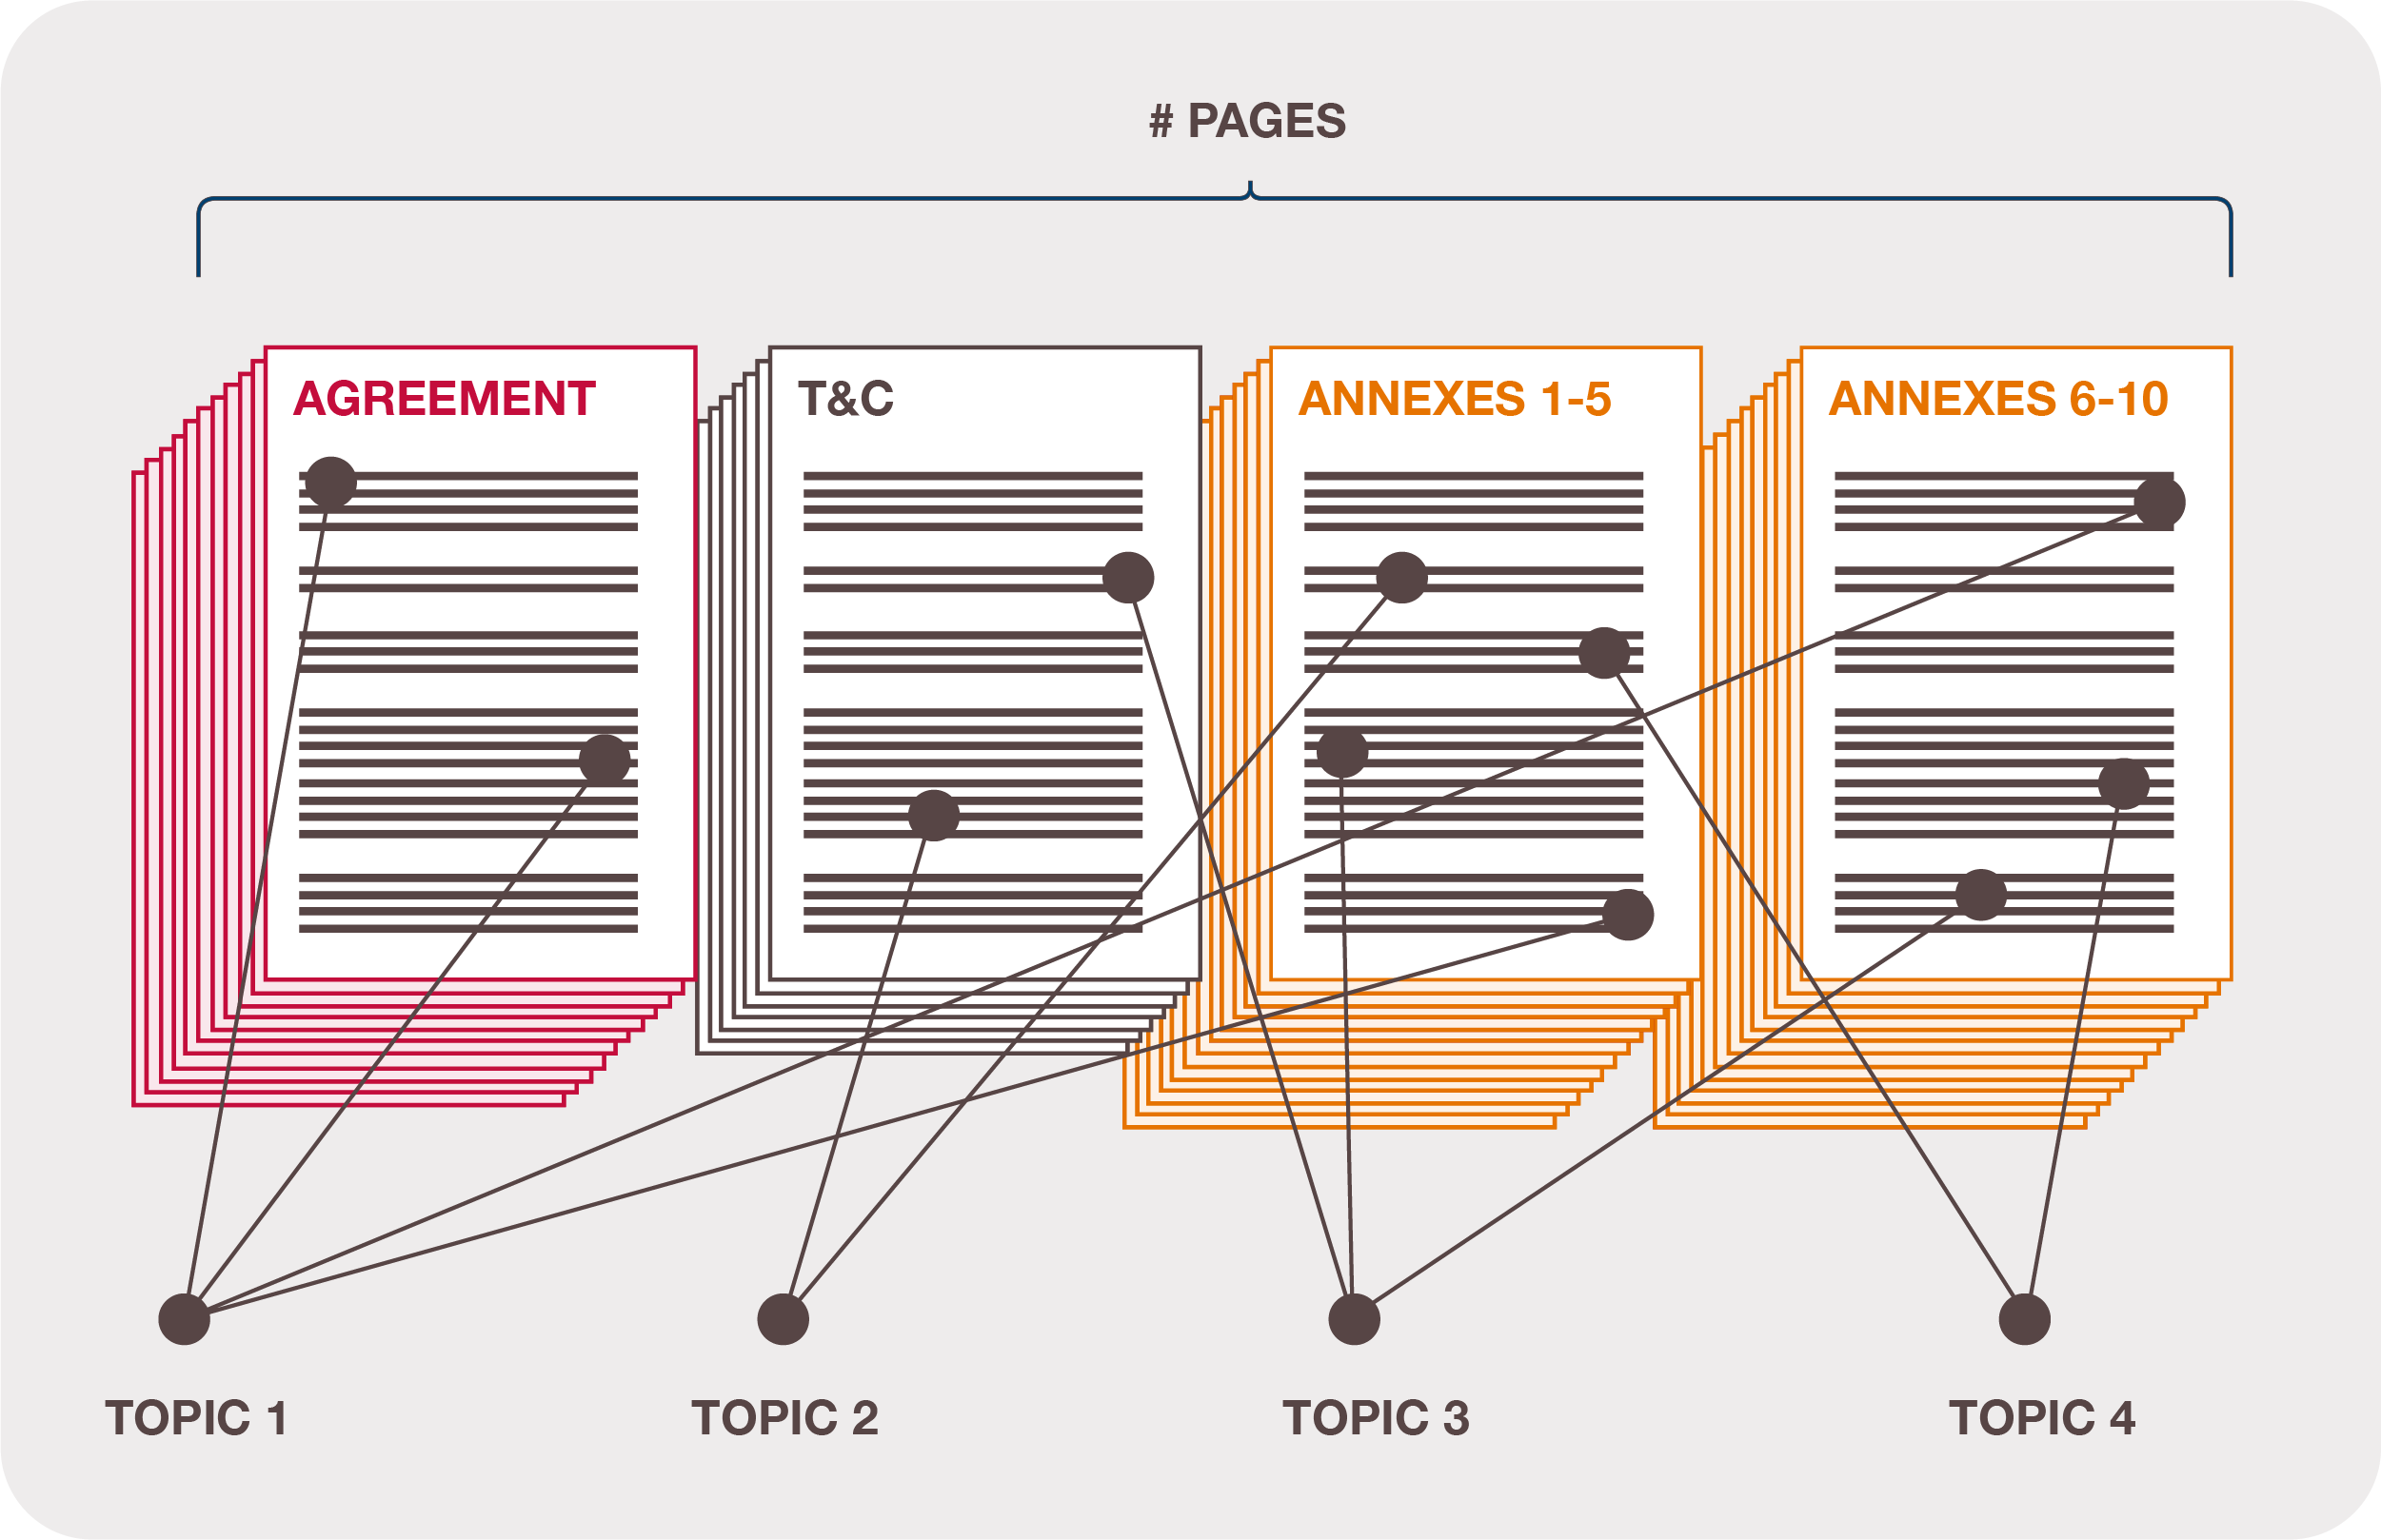
\includegraphics[width=0.6\textwidth]{image.png}
    \caption{Contract document mapping visualization.}
    \textit{{Source}: World Commerce \& Contracting, https://contract-design.worldcc.foundation/contract-doc-map}
    \label{fig:contract-doc-map}
\end{figure}



\section*{Related Work}
Existing datasets such as the CUAD dataset by the Atticus Project and the Stanford ContractNLI dataset have paved the way for legal contract analysis in NLP.\@ However, many existing datasets focus on broad contract types, leaving gaps in specific clause identification and domain-specific labeling. Our dataset will build upon these works while addressing these gaps, ensuring more comprehensive contract clause categorization.


\section*{Proposed Work}
We will develop a structured pipeline for contract clause labeling, leveraging a combination of:

\begin{itemize}
	\item Existing contract datasets (e.g., CUAD, ContractNLI)
	\item Manual annotation by legal experts
	\item Automated preprocessing and classification methods
\end{itemize}


This dataset will support model training for clause classification, summarization, and quality evaluation of contracts. The dataset creation process will be documented to ensure reproducibility and scalability.

\section*{Datasets}
Our dataset will integrate data from:

\begin{itemize}
	\item CUAD dataset (labeled contract clauses for NLP applications)
	\item Stanford ContractNLI dataset (legal contract entailment tasks)
	\item Other publicly available legal contract corpora
	\item Manually labeled contracts for our specific use case (to be defined)
\end{itemize}

We will ensure diversity in contract types and ensure annotations align with real-world contract analysis needs.

\section*{Evaluation}
We will evaluate our dataset and labeling methodology based on:

\begin{itemize}
	\item Inter-annotator agreement scores for manual labels
	\item Benchmarking against existing datasets in clause classification tasks
	\item Model performance on clause categorization and summarization tasks using our dataset
\end{itemize}

Success will be determined by achieving high consistency in annotations and improved model performance compared to existing models on existing and currated datasets.

\section*{Timeline}
\begin{itemize}
	\item Week 1-2: Research best practices in contract dataset creation, including fairness metrics, contract usefulness, and aggregation methods.
	\item Week 3-4: Investigate clause polarity (evaluating if a clause is beneficial or detrimental) and define quantifiable measures for fairness.
	\item Week 5-6: Explore classification approaches for contract clauses and analyze potential legal loopholes in existing datasets.
	\item Week 7-8: Collect and preprocess contract samples, ensuring a balanced representation across different contract types.
	\item Week 9-10: Perform k-means-based semi-automated labeling, clustering contract clauses based on semantic similarities to predefined categories. Also explore dynamic categorization with k-means.
	\item Week 11: Validate dataset quality through inter-annotator agreement and benchmark dataset performance using AI models.
	\item Week 12: Finalize dataset, prepare documentation, and determine dataset effectiveness with domain experts.
\end{itemize}
\section*{Conclusion}
Our project aims to fill a crucial gap in legal NLP by creating a high-quality labeled dataset of contract clauses. By ensuring accurate categorization and annotation, we will contribute to the advancement of AI-driven contract analysis tools, ultimately fostering better legal transparency and compliance.

\begin{thebibliography}{9}

	\bibitem{cuad}
	The Atticus Project.
	\textit{CUAD: Contract Understanding Atticus Dataset, https://www.atticusprojectai.org/cuad}.
	Accessed 26 Mar. 2025.
	
	\bibitem{contractnli}
	Stanford NLP Group.
	\textit{ContractNLI: A Benchmark for Legal Contract Entailment, https://stanfordnlp.github.io/contract-nli/}.
	Accessed 26 Mar. 2025.

	\bibitem{image}
	World Commerce \& Contracting.
	\textit{Contract design pattern library, https://contract-design.worldcc.foundation/library}.
    Accessed 26 Mar. 2025.

	\end{thebibliography}
\end{document} 

